\documentclass[11pt]{article}
\usepackage{comment}
\usepackage{graphicx}
\usepackage{fourier-orns}
\usepackage{algorithm, algpseudocode} % For pseudo code
\usepackage{tabto}
\usepackage{amsmath, amsthm, amssymb, amsfonts} % Linear algebra and logic related symbols
\usepackage{color}
\usepackage{fancyhdr} % Header
\usepackage{enumitem} % More option for enumeration and itemization
%\usepackage{palatino} % font
\usepackage{latexsym}
\usepackage{fourier-orns}
\usepackage{algorithm, algpseudocode} % For pseudo code
\usepackage{tabto}
\usepackage{amsmath, amsthm, amssymb, amsfonts}
\usepackage{color}
\usepackage{fancyhdr} % Header
\usepackage{enumitem} % More option for enumeration and itemization
\usepackage{tikz}
\usetikzlibrary{arrows} % graph
\usepackage{url}
\topmargin=-.5in    %0cm
\textheight=9.0in     %24.1cm            
\evensidemargin=0in %0cm
\oddsidemargin=0.0in  %-.3cm
\textwidth=6.5in    %16.5cm 

\title{CS182 Homework \# 1}
\author{Your Name}
\date{\today}

\begin{document}

\maketitle

%\section{Introduction}

\begin{enumerate}
    \item %Change John Doe to your first and last name
    \begin{quote}
    \textit{I, Maninder (Kaurman) Kaur, affirm that I have not given or received any unauthorized help on this assignment and that this work is my own. What I have submitted is expressed and explained in my own words. I have not used any online websites that provide a solution. I will not post any parts of this problem set to any online platform and doing so is a violation of course policy.}
    \end{quote}

    %Use \clearpage for starting a new page
    \clearpage
    \item Common notations: $\leq$, $<$, $\geq$, $>$, $a\equiv b \pmod{n}$, $x^y$, $a_5$, $x\bmod{n} = r$, $x={p \over q}$

    Quantifiers: $\forall$, $\exists$
    
$$\text{Matrix: }\left[\begin{array}{cc}a & b \cr c & d\end{array}\right]$$
Table:
\begin{center}
 \begin{tabular}{| c | c | c | c |c |c |c|} 
 \hline
 p & q & r & $\neg r$ & $q \rightarrow  r$ & $p \wedge (q \rightarrow r)$ & $p\wedge (q\rightarrow r)\leftrightarrow \neg r$\\ [0.5ex] 
 \hline\hline
  F & F& F &  &  &  & \\ 
 \hline
  F & F& T &  &  &  &\\ 
 \hline
  F & T& F &  & &  &  \\ 
 \hline
  F & T& T &  &  & & \\ 
 \hline
  T & F& F&  &  &  & \\ 
 \hline
  T & F& T &  &  &  & \\ 
 \hline
  T & T & F &  &  &  & \\ 
 \hline
  T & T& T &  &  &  & \\ 
 \hline
\end{tabular}
\end{center}

Integral and Summations:
$$\int_{-\infty}^{\infty}e^{-x^2}\ dx = \sqrt{\pi},\quad \quad \sum_{n=1}^{\infty}{1\over n^2}={\pi^2 \over 6}$$

    \clearpage
    \item Example of a multi-part question.

    %Use [label=(\alph*)] for part (a), part (b) labeling
    \begin{enumerate}[label=(\alph*)]
        \item $((p \lor (q \rightarrow \neg p))\land (p\lor(\neg q\rightarrow p))) \lor (p\rightarrow q)$
        \item $\neg(\neg q\lor (\neg(\neg q\land p)\land q))\land p$
        \item $(p\rightarrow q)\land(q\rightarrow\neg p)$
    \end{enumerate}

    \textit{Solution.}

    \begin{enumerate}[label=(\alph*)]
        \item 
        \item 
        \item 
    \end{enumerate}

    \clearpage
    \item 
    \begin{equation*}
        \begin{split}
            S_n &= 1+2+\cdots+n \\
            &= {n(n+1)\over 2}
            %an example of math equation, this is a comment in LaTeX
        \end{split}
    \end{equation*}

    %This is a comment in LaTeX. Below is the format you should use when writing logical equivlance equations.
    
    \begin{align*}
        p \lor (q \lor r) &\equiv (p \lor q) \lor r & \text{Associative Law}\\
        &\equiv p \lor (q \land r) & \text{Associative Law}
    \end{align*}

    \clearpage
    \item This is an example of using tikz to draw an undirected graph.
    
        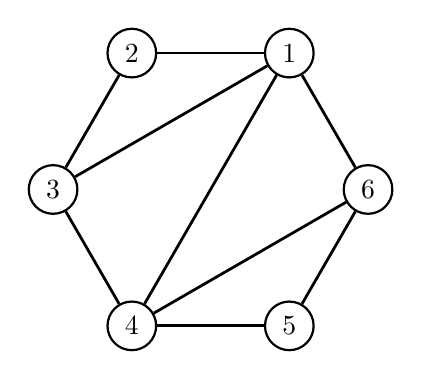
\begin{tikzpicture}
            \foreach \i/\label in {1, 2, 3, 4, 5, 6} {
              \node[draw, circle, fill=white, thick] (v\label) at (360/6*\i:2) {\label};
            }
            \draw[-, line width=1pt, >=latex] 
            (v1) -- (v2);
            \draw[-, line width=1pt, >=latex] (v1) -- (v4);
            \draw[-, line width=1pt, >=latex] (v2) -- (v3);
            \draw[-, line width=1pt, >=latex] (v3) -- (v4);
            \draw[-, line width=1pt, >=latex] (v4) -- (v5);
            \draw[-, line width=1pt, >=latex] (v5) -- (v6);
            \draw[-, line width=1pt, >=latex] (v6) -- (v1);
            \draw[-, line width=1pt, >=latex] (v1) -- (v3);
            \draw[-, line width=1pt, >=latex] (v4) -- (v6);
        \end{tikzpicture}

    This is an example of using tikz to draw a directed graph.

    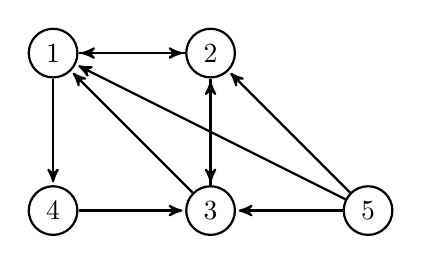
\begin{tikzpicture}[->, >=stealth', shorten >=1pt, auto, node distance=2cm, thick, main node/.style={circle, draw, fill=white!20}]
        % Nodes
        \node[main node] (1) {1};
        \node[main node] (2) [right of=1] {2};
        \node[main node] (3) [below of=2] {3};
        \node[main node] (4) [below of=1] {4};
        \node[main node] (5) [right of=3] {5};

        % Arrows/Edges to match the indegrees and outdegrees
        \path[every node/.style={font=\sffamily\small}]
        (5) edge (2)
            edge (3)
            edge (1)
        (4) edge (3)
        (3) edge (2)
            edge (1)
        (2) edge (3)
            edge (1)
        (1) edge (4)
            edge (2);
    \end{tikzpicture}

\end{enumerate}

\end{document}

